\section{Weight sharing}

\subsection{Proposed convolution operator}
\label{operator}
  \subsubsection{Definitions}

Let $S$ be a set of points, such that each one defines a set of neighbourhoods.

An \textit{entry} $e$ of a \textit{dataset} $\mathcal{D}$ is a column vector that can be of any size, for which each dimension represents a \textit{value taken by $e$} at a certain point $u \in S$. $u$ is said to be \textit{activated} by $e$. A point $u$ can be associated to at max one dimension of $e$. If it is the $i$th dimension of $e$, then we denote the value taken by $e$ at $u$ by either $e_u$ or $e_i$. $\mathcal{D}$ is said to be \textit{embedded} in $S$.

We say that two entries $e$ and $e'$ are \textit{homogeneous} if they have the same size and if their dimensions are always associated to the same points.

  \subsubsection{Formal description of the \textit{generalized} convolution}

Let's denote by $\mathcal{C}$ a generalized convolution operator.We want it to observe the following conditions:
\begin{itemize}
  \item Linearity
  \item Locality
  \item Kernel weight sharing
\end{itemize}

As $\mathcal{C}$ must be linear, then for any entry $e$, there is a matrix $W^e$ such that $\mathcal{C}(e) = W^ee$. Note that unless the entries were all homogeneous, $W^e$ depends on $e$.

In order to meet the locality condition, we first want that the coordinates of $\mathcal{C}(e)$ have a local meaning. To this end, we impose that $\mathcal{C}(e)$ lives in the same space than $e$, and that $\mathcal{C}(e)$ and $e$ are homogeneous. Secondly, for each $u$, we want $\mathcal{C}(e)_u$ to be only function of values taken by $e$ at points contained in a certain neighbourhood of $u$. It results that lines of $W^e$ are generally sparse.

Let's attribute to $\mathcal{C}$ a kernel of $n$ weights in the form of a row vector $w = (w_1,w_2,..,w_n)$, and let's define the set of allocation matrices $\mathcal{A}$ as the set of binary matrices that have at most one non-zero coordinate per column. As $\mathcal{C}$ must share its weights across the activated points, then for each row $W^e_i$ of $W^e$, there is an allocation matrix $A^e_i \in \mathcal{A}$ such that $W^e_i = wA^e_i$. To maintain locality, the $j$th column of $A^e_i$ must have a non-zero coordinate if and only if the $i$th and $j$th activated points are in a same neighbourhood.

Let's $A^e$ denotes the block column vector that has the matrices $A^e_i$ for attributes, and let's $\otimes$ denotes the tensor product. Hence, $\mathcal{C}$ is defined by a weight kernel $w$ and an allocation map $e \mapsto A^e$ that maintains locality, such that
\begin{align}
\mathcal{C}(e) = (w \otimes A^e)\ .\ e
\end{align}

  \subsubsection{Generalized convolution supported by an underlying graph}

As vertices, the set of activated points of an entry $e$ defines a complete oriented graph that we call $G^e$. If all the entries are homogeneous, then $G^e$ is said to be \textit{static}. In this case, we note $G$.

Suppose we are given $u \mapsto \mathcal{V}_u$ which maps each $u \in S$ to a neighbourhood $\cn_u$. We then define  $G^e_\cn$ as the subgraph of $G^e$ such that it contains the edge $(u',u)$ if and only if $u' \in \cn_{u}$. Let $a_\cn: e \mapsto A^e$ be an allocation map such that the $j$th column of $A^e_i$ have a non-zero coordinate if and only if $(e_i,e_j)$ is an edge of $G^e_\cn$.

Then the generalized convolution of $e$ by the couple $(w,a_\cn)$ is supported by the underlying graph $G^e_\cn$ in the sense that $W^e_\cn = w \otimes a_\cn(e)$ is its adjacency matrix. Note that the underlying graph of a regular convolution is a lattice and its adjacency matrix is a Toëplitz matrix.

Also note that the family $(\mathcal{V}_u)_{u \in S}$ can be seen as local receptive fields for the generalized convolution, and that the map $a_\cn$ can be seen as if it were distributing the kernel weights into each $\mathcal{V}_u$.\\

  \paragraph{Remarks}

The generalized convolution has been defined here in view of being applied to the CNN paradigm, i.e. as an operation between a kernel weight and a vector. In the context of graph signal processing, if $G=(E,V)$ denotes a graph, then such operator $\ast$ with respect to the 3D tensor $A$ between two graph signals $f, g \in \mathbb{R}^E$ would have been defined as:
\begin{align}
f \ast g &= (f^\top \otimes A)\ .\ g\\
\forall v \in V,\ (f \ast g)(v) &= f^\top A_v\ g, \textit{ with } A_v \in \mathcal{A}
\end{align}\\ 
Note that in our context, the underlying graph depends on the entry. So that if the generalized convolution is placed inside a deep neural network architecture (see section~\ref{cnn}), then the learnt filter $w$ will be reusable regardless of the entry's underlying structure. 

  \subsubsection{Example of a generalized convolution shaped by a rectangular window}
\label{rectangle}

Let $\bbe$ be a two-dimensional Euclidean space and let's suppose here that $S = \bbe$.

Let's denote by $\mathcal{C_\mathcal{R}}$, a generalized convolution shaped by a rectangular window $\mathcal{R}$. We suppose that its weight kernel $w$ is of size $N_w = (2p+1)(2q+1)$ and that $\mathcal{R}$ is of width $(2p+1)\mu$ and height $(2q+1)\mu$, where $\mu$ is a given unit scale.

Let $G^e_{p,q}$ be the subgraph of $G^e$ such that it contains the edge $(u',u)$ if and only if $|u'_x-u_x| \leq (p + \frac{1}2)\mu$ and $|u'_y-u_y| \leq (q + \frac{1}2)\mu$. In other terms, $G^e_{p,q}$ connects a vertex $u$ to every vertex contained in $\mathcal{R}$ when centered on $u$.

Then, we define $\mathcal{C_\mathcal{R}}$ as being supported by $G^e_{p,q}$. As such, its adjacency matrix acts as the convolution operator. At this point, we still need to affect the kernel weights to its non-zero coordinates, via the edges of $G^e_{p,q}$. This amounts for defining explicitely the map $e \mapsto A^e$ for $\mathcal{C_\mathcal{R}}$. To this end, let's consider the grid of same size as that rectangle, which breaks it down into $(2p+1)(2q+1)$ squares of side length $\mu$, and let's associate a different weight to each square. Then, for each edge $(u',u)$, we affect to it the weight associated with the square within which $u'$ falls when the grid is centered on $u$. This procedure allows for the weights to be shared across the edges. It is illustrated on figure~\ref{irrDomain}.

Note that if the entries are homogeneous and the activated points are vertices of a regular grid, then the matrix $W$, independant of $e$, is a Toëpliz matrix which acts as a regular convolution operator on the entries $e$. In this case, $\mathcal{C_\mathcal{R}}$ is just a regular convolution. For example, this is the case in section~\ref{link}.

\begin{figure}[h]
  \begin{floatrow}
    \ffigbox{
      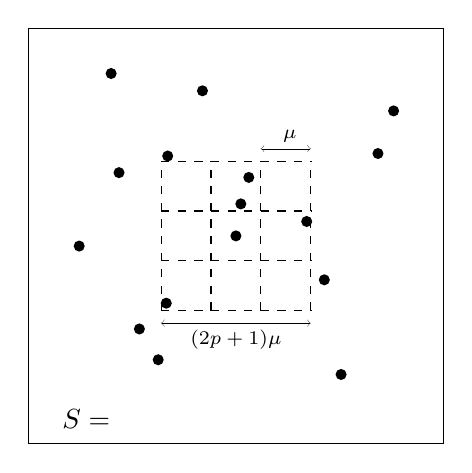
\begin{tikzpicture}[scale=1.055]
        \pgfmathsetseed{333}
        \tikzstyle{every node}= [circle,fill=black, minimum size= 4pt,inner sep=0pt];
        \foreach \x in {1,2,4}{
          \foreach \y in {1,2,3,4}{
            \node(\x\y) at (\x+0.5*rand,\y+0.5*rand) {};
          }
        }
        \foreach \y in {1,2,4}{
            \node(3\y) at (3+0.5*rand,3+0.5*rand) {};
        }
        \node(33)[circle,fill=black] at (2.5,2.5) {};
        \foreach \x in {1.6,2.2,2.8,3.4}{
          \path[dashed]
          (\x,1.6) edge (\x,3.4)
          (1.6,\x) edge (3.4,\x);
        }

        \draw[ultra thin] (1.6,1.45) edge[<->] (3.4,1.45);
        \draw[ultra thin] (2.8,3.55) edge[<->] (3.4,3.55);
        \node[draw=none,fill=none] at (2.5,1.25) {\scriptsize{$(2p+1)\mu$}};
        \node[draw=none,fill=none] at (3.15,3.7) {\scriptsize{$\mu$}};

        \draw (0,0) rectangle (5,5);
        \node[draw=none,fill=none] at (0.7,0.3) {$S=\bbe$};
      \end{tikzpicture}
    }
    {
      \caption{Example of a moving grid. The grid defines the allocation of the kernel weights.}
      \label{irrDomain}
    }
    \ffigbox{
      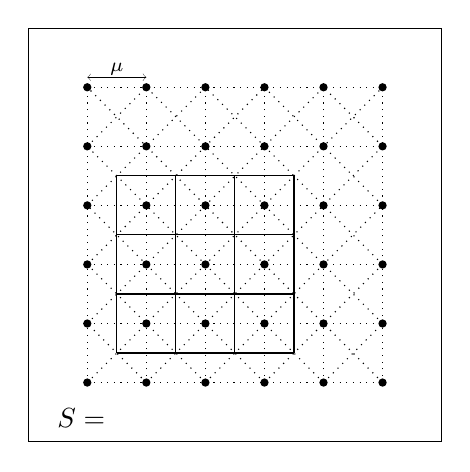
\begin{tikzpicture}[scale=0.75]
        \tikzstyle{every node}= [circle,fill=black, minimum size= 3pt,inner sep=0pt];
          \foreach \x in {1,2,3,4,5,6}{
            \foreach \y in {1,2,3,4,5,6}{
              \node(\x\y) at (\x,\y) {};
            }
          }

          \foreach \x in {1.5,2.5,3.5,4.5}{
            \path[thin]
            (\x,1.5) edge (\x,4.5)
            (1.5,\x) edge (4.5,\x);
          }

          \draw[ultra thin] (1,6.17) edge[<->] (2,6.17);
          \node[draw=none,fill=none] at (1.5,6.3) {\scriptsize{$\mu$}};

          \foreach \x in {1,2,3,4,5,6}{
            \draw[dotted,thin] (1,\x) -- (6,\x);
            \draw[dotted,thin] (\x,1) -- (\x,6);
          }

          \foreach \x in {1,2,3,4,5}{
            \draw[dotted,thin] (1,\x) -- (7-\x,6);
            \draw[dotted,thin] (6,\x) -- (\x,6);
          }

          \foreach \x in {2,3,4,5}{
            \draw[dotted,thin] (\x,1) -- (6,7-\x);
            \draw[dotted,thin] (7-\x,1) -- (1,7-\x);
          }

          \draw (0,0) rectangle (7,7);

          \node[draw=none,fill=none] at (0.9,0.4) {$S=\bbe$};
      \end{tikzpicture}
    }
    {
      \caption{On regular domains, the moving grid allocates the weights similarly to the moving window of a standard convolution.}
      \label{regDomain}
    }
  \end{floatrow}
\end{figure}

  \subsubsection{Link with the standard convolution on image datasets}
  \label{link}

  Let $\mathcal{D}$ be an image dataset. Entries of $\mathcal{D}$ are homogeneous and their dimensions represent the value at each pixel. In this case, we can set $S=\bbe$, of dimension 2, such that each pixel is located at entire coordinates. More precisely, if the images are of width $n$ and height $m$, then the pixels are located at coordinates $(i,j) \in \{0, 1, 2, ..., n\} \text{x} \{0, 1, 2, ..., m\}$. Hence, the pixels lie on a regular grid and thus are spaced out by a constant distance $\mu = 1$.

  Let's consider the static underlying graph $G_{p,q}$ and the generalized convolution by a rectangular window $\mathcal{C_\mathcal{R}}$, as defined in the former section. Then, applying the same weight allocation strategy will lead to affect every weight of the kernel into the moving window $\mathcal{R}$. Except on the border, one and only one pixel will fall into each square of the moving grid at each position, as depicted in figure~\ref{regDomain}. Indeed, $\mathcal{R}$ behaves exactly like a moving window of the standard convolution, except that it considers that the images are padded with zeroes on the borders.

  \subsection{Application to CNNs}
\label{cnn}

  \subsubsection{Neural network interpretation}

Let $\mathcal{L}^d$ and $\mathcal{L}^{d+1}$ be two layers of neurons, such that forward-propagation is defined from $\mathcal{L}^d$ to $\mathcal{L}^{d+1}$. Let's define such layers as a set of neurons being located in $S$. These layers must contain as many neurons as points that can be activated. In other terms, $S \cong \mathcal{L}^d \cong \mathcal{L}^{d+1}$. As such, we will abusively use the term of \textit{neuron} instead of \textit{point}.

  \begin{figure}[h]
  \centering
  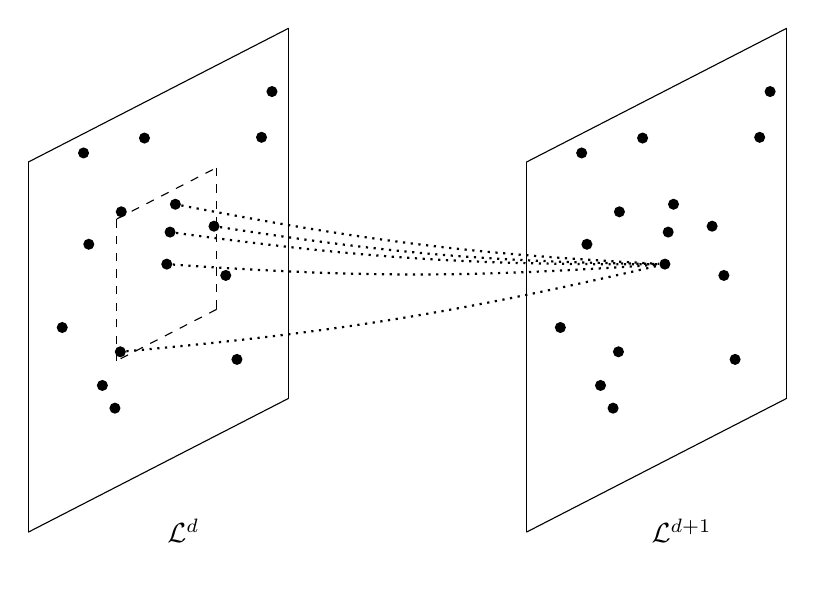
\begin{tikzpicture}
  
\newcommand{\nnn}{4.7}
  \begin{scope}[rotate around y = 70]
\pgfmathsetseed{333}
\tikzstyle{every node}= [circle,fill=black, minimum size= 4pt,inner sep=0pt];
    \foreach \x in {1,2,4}{
      \foreach \y in {1,2,3,4}{
        \node(\x\y) at (\x+0.5*rand,\y+0.5*rand) {};
      }
    }
    \foreach \y in {1,2,4}{
        \node(3\y) at (3+0.5*rand,3+0.5*rand) {};
    }
    \node(33)[circle,fill=black] at (2.5,2.5) {};
      \path[dashed]
      (1.6,1.6) edge (1.6,3.4)
      (1.6,3.4) edge (3.4,3.4)
      (3.4,3.4) edge (3.4,1.6)
      (3.4,1.6) edge (1.6,1.6);

    \path[thin]
      (0,0) edge (0,\nnn)
      (0,\nnn) edge (\nnn,\nnn)
      (0,0) edge (\nnn,0)
      (\nnn,0) edge (\nnn,\nnn);

    \node[draw=none,fill=none] at (2.8,-1) {$\mathcal{L}^d$};
    \end{scope}
  \begin{scope}[xshift=180pt,rotate around y = 70]
\pgfmathsetseed{333}
\tikzstyle{every node}= [circle,fill=black, minimum size= 4pt,inner sep=0pt];
    \foreach \x in {1,2,4}{
      \foreach \y in {1,2,3,4}{
        \node(\x\y') at (\x+0.5*rand,\y+0.5*rand) {};
      }
    }
    \foreach \y in {1,2,4}{
        \node(3\y') at (3+0.5*rand,3+0.5*rand) {};
    }
    \node(33')[circle,fill=black] at (2.5,2.5) {};

    \path[thin]
      (0,0) edge (0,\nnn)
      (0,\nnn) edge (\nnn,\nnn)
      (0,0) edge (\nnn,0)
      (\nnn,0) edge (\nnn,\nnn);

    \node[draw=none,fill=none] at (2.8,-1) {$\mathcal{L}^{d+1}$};
  \end{scope}

\draw[dotted,thick,-] (33) edge[bend right=4] (33');
\draw[dotted,thick,-] (22) edge[bend right=4] (33');
\draw[dotted,thick,-] (32) edge[bend right=4] (33');
\draw[dotted,thick,-] (34) edge[bend right=4] (33');
\draw[dotted,thick,-] (31) edge[bend right=4] (33');

  \end{tikzpicture}
  \caption{Generalized convolution between two layers of neurons.}
  \label{nn}
\end{figure}

The \textit{generalized} convolution between these two layers can be interpreted as follow. An entry $e$ activates the same $N$ neurons in each layer. Then, a convolution shape takes $N$ positions onto $\mathcal{L}^d$, each position being associated to one of the activated neurons of $\mathcal{L}^{d+1}$. At each position, connections are drawn from the activated neurons located inside the convolution shape in destination to the associated neuron. And a subset of weights from $w$ are affected to these connections, according to a weight sharing strategy defined by an allocation map. Figure~\ref{nn} illustrates a convolution shaped by a rectangular window.

The forward and backward propagation between $\mathcal{L}^d$ and $\mathcal{L}^{d+1}$  are applied using the described neurons and connections. After a generalized convolution operation, an activation function is applied on the output neurons. Then a pooling operation is done spatially: the input layer is divided into patches of same size, and all activated neurons included in this patch are pooled together. Unlike a standard pooling operation, the number of activated neurons in a patch may vary.

Indeed, generalized convolution layers can be vectorized. They can have multiple input channels and multiple feature maps. They shall naturally be placed into the same kind of deep neural network structure than in a CNN. Thus, they are for the irregular input spaces what the standard convolution layers are for regular input spaces.

  \subsubsection{Implementation}

There are two main strategies to implement the propagations. The first one is to start from (1), derive it and vectorize it. It implies handling semi-sparse representations to minimize memory consumption and to use adequate semi-sparse tensor products.

Instead, we decide to use the neural network interpretation and the underlying graph structure whose edges amount for neurons connections. By this mean, the sparse part of the computations is included via the use of this graph. Also, computations on each edge can be parallelized.

  \subsubsection{Forward and back propagation formulae}
  \label{formulae}

Let's first recall the propagation formulae from a neural network point of view.

Let's denote by $e_u$ the value of a neuron of $\mathcal{L}^d$ located at $u \in S$, by $f_v$ for a neuron of $\mathcal{L}^{d+1}$, and by $g_v$ if this neuron is activated by the activation function $\sigma$.

We denote by $\textit{prev}(v)$ the set neurons from the previous layer connected to $v$, and by $\textit{next}(u)$ those of the next layer connected to $u$. $\textit{w}_{uv}$ is the weight affected to the connection between neurons $u$ and $v$. $b$ is the bias term associated to $\mathcal{L}^{d+1}$.

After the forward propagation, values of neurons of $\mathcal{L}^{d+1}$ are determined by those of $\mathcal{L}^d$:
\begin{align}
f_v &= \sum_{u \in \textit{prev}(v)}{e_u\textit{w}_{uv}} \\
g_v &= \sigma(f_v + b)
\end{align}

Thanks to the chain rule, we can express derivatives of a layer with those of the next layer:
\begin{align}
\delta_v = \frac{\partial{E}}{\partial{f_v}} &= \frac{\partial{E}}{\partial{g_v}}\frac{\partial{g_v}}{\partial{f_v}} = \frac{\partial{E}}{\partial{g_v}}\sigma^{'}(f_v + b) \\
\frac{\partial{E}}{\partial{e_u}} &= \sum_{v \in \textit{next(u)}}{\frac{\partial{E}}{\partial{f_v}}\frac{\partial{f_v}}{\partial{e_u}}} = \sum_{v \in \textit{next(u)}}{\delta_v\textit{w}_{uv}}
\end{align}

We call $\textit{edges}(\textit{w})$ the set of edges to which the weight $\textit{w}$ is affected. If $\omega \in \textit{edges}(\textit{w})$, $f_{\omega^+}$ denotes the value of the destination neuron, and $e_{\omega^-}$ denotes the value of the origin neuron.

The back propagation allows to express the derivative of any weight $\textit{w}$:
\begin{align}
\frac{\partial{E}}{\partial{\textit{w}}} &= \sum_{\omega \in \textit{edges}(\textit{w})}{\frac{\partial{E}}{\partial{f_{\omega^+}}}\frac{\partial{f_{\omega^+}}}{\partial{\textit{w}}}} = \sum_{\omega \in \textit{edges}(\textit{w})}{\delta_{\omega^+}e_{\omega^-}} \\
\frac{\partial{E}}{\partial{b}} &= \sum_{v}{\frac{\partial{E}}{\partial{g_v}}\frac{\partial{g_v}}{\partial{b}}} = \sum_{v}{\delta_v}
\end{align}

The sets $\textit{prev}(v)$, $\textit{next}(u)$ and $\textit{edges}(\textit{w})$ are determined by the graph structure, which in turn is determined beforehand by a procedure like the one described in section~\ref{rectangle}.

  \subsubsection{Vectorization}

Computations are done per batch of entries $B$. Hence, the graph structure used for the computations must contain the weighted edges of all entries $e \in B$. If necessary, entries of $B$ are made homogeneous: if a neuron $u$ is not activated by an entry $e$ but is activated by another entry of $B$, then $e_u$ is defined and is set to zero.

The 3D tensor counterparts of $e$, $f$, and $g$ are thus denoted by $\mathscr{E}$, $\mathscr{F}$ and $\mathscr{G}$. Their third dimension indexes the channels (input channels or feature maps). Their submatrix along the neuron located at $x \in S$ are denoted $\mathscr{E}_x$, $\mathscr{F}_x$ and $\mathscr{G}_x$, rows are indexing entries and columns are indexing channels.
The counterparts of $\textit{w}$ and $b$ are $\mathscr{W}$ and $\beta$. The first being a 3D tensor and the second being a vector with one value per feature map. $\widetilde{\beta}$ denotes the 3D tensor obtained by broadcasting $\beta$ along the two other dimensions of $\mathscr{F}$. $\mathscr{W}_\textit{w}$ denotes the submatrix of $\mathscr{W}$ along the kernel weight $\textit{w}$. Its rows index the feature maps and its columns index the input channels.

With these notations, the vectorized counterparts of the formulae from section~\ref{formulae} can be obtained in the same way:
\begin{align}
\mathscr{F}_v &= \sum_{u \in \textit{prev}(v)}{\mathscr{E}_u\mathscr{W}_{\textit{w}_{uv}}^\top} \\
\mathscr{G} &= \sigma(\mathscr{F} + \widetilde{\beta}) \\
\Delta = \left(\frac{\partial{E}}{\partial{\mathscr{F}}}\right) &= \left(\frac{\partial{E}}{\partial{\mathscr{G}}}\right)\circ\ \sigma^{'}(\mathscr{F} + \widetilde{\beta}) \\
\left(\frac{\partial{E}}{\partial{\mathscr{E}}}\right)_u &= \sum_{v \in \textit{next(u)}}{\Delta_v\mathscr{W}_{uv}} \\
\left(\frac{\partial{E}}{\partial{\mathscr{W}}}\right)_\textit{w} &= \sum_{\omega \in \textit{edges}(\textit{w})}{\Delta_{\omega^+}^\top\mathscr{E}_{\omega^-}} \\
\frac{\partial{E}}{\partial{\beta}} &= \sum_{j}{\left(\sum_{v}{\Delta_v}\right)_{j\textit{-th column}}}
\end{align}

Where $\circ$ and $^\top$ respectively denotes Hadamard product and transpose.

\subsection{Experiments}
\label{experiments}
  %\subsubsection{Sanity check on regular image lattice}
  %\subsubsection{Distorded MNIST}
  %\subsubsection{Human activity recognition}

In order to measure the gain of performance allowed by the generalized CNN over MLP  on irregular domains, we made a series of benchmarks on distorded versions of the MNIST dataset~\cite{lecun1998mnist}, consisting of images of 28x28 pixels. To distort the input domain, we plunged the images into a 2-d euclidean space by giving entire coordinates to pixels. Then, we applied a gaussian displacement on each pixel, thus making the data irregular and unsuitable for regular convolutions. For multiple values of standard deviation of the displacement, we trained a generalized CNN and compared it with a MLP that has the same number of parameters. We choosed a simple yet standard architecture in order to better see the impact of generalized layers.

The architecture used is the following: a generalized convolution layer with relu~\cite{glorot2011deep} and max pooling, made of 20 feature maps, followed by a dense layer and a softmax output layer. The generalized convolution is shaped by a rectangular window of width and height $5\mu$ where the unit scale $\mu$ is chosen to be equal to original distance between two pixels. The max-pooling is done with square patches of side length $2\mu$. The dense layer is composed of 500 hidden units and is terminated by relu activation as well. In order to have the same number of parameters, the compared MLP have 2 dense layers of 500 hidden units each and is followed by the same output layer. For training, we used stochastic gradient descent~\cite{bottou2010large} with Nesterov momentum~\cite{sutskever2013importance} and a bit of L2 regularization~\cite{ng2004feature}.% Both architectures are trained on 15 epochs.

\begin{figure}[!h]
  \centering
  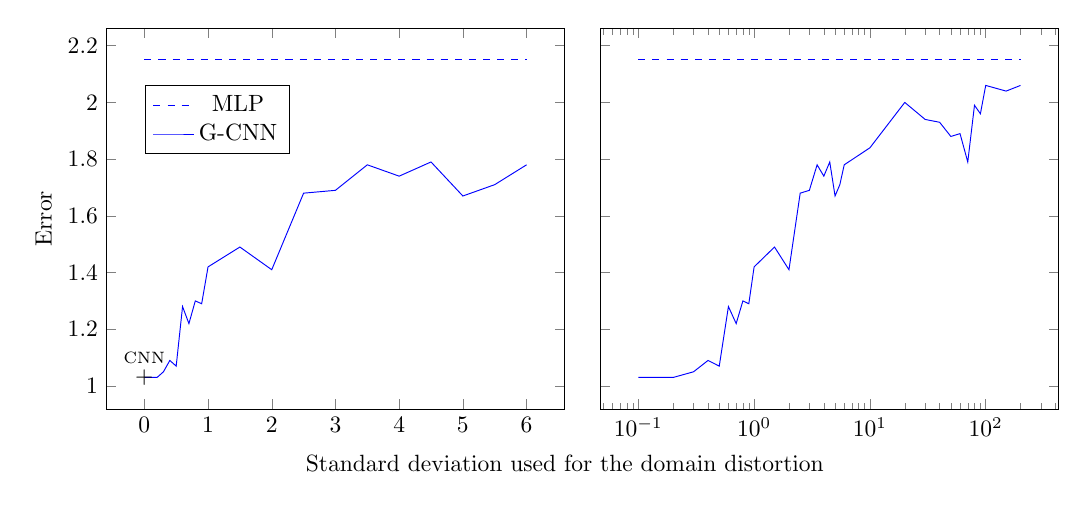
\begin{tikzpicture}[scale=0.85]
    \begin{axis}[ xlabel=Standard deviation used for the domain distortion, ylabel=Error,
      legend style={at={(0.4,0.85)}, anchor=north east},
      x label style={at={(axis description cs:1,-0.1)},anchor=north}]

      \addplot[color=blue,dashed,mark=.] coordinates {
        (0.0, 2.15) (6.0, 2.15)
      };

      \addplot[color=blue,mark=.] coordinates {
      (0.0, 1.03)
      (0.1, 1.03)
      (0.2, 1.03)
      (0.3, 1.05)
      (0.4, 1.09)
      (0.5, 1.07)
      (0.6, 1.28)
      (0.7, 1.22)
      (0.8, 1.30)
      (0.9, 1.29)
      (1.0, 1.42)
      (1.5, 1.49)
      (2.0, 1.41)
      (2.5, 1.68)
      (3.0, 1.69)
      (3.5, 1.78)
      (4.0, 1.74)
      (4.5, 1.79)
      (5.0, 1.67)
      (5.5, 1.71)
      (6.0, 1.78)
      };

      \node at (0.0, 1.03) {+};
      \node at (0.0, 1.10) {\scriptsize{CNN}};

      \legend{MLP, G-CNN}
    \end{axis}

    \begin{scope}[xshift = 210pt]
      \begin{semilogxaxis}[yticklabels={,,}]

        %\node at (0.1, 1.49) {+};

        \addplot[color=blue,mark=.] coordinates {
        (0.0, 1.03)
        (0.1, 1.03)
        (0.2, 1.03)
        (0.3, 1.05)
        (0.4, 1.09)
        (0.5, 1.07)
        (0.6, 1.28)
        (0.7, 1.22)
        (0.8, 1.30)
        (0.9, 1.29)
        (1.0, 1.42)
        (1.5, 1.49)
        (2.0, 1.41)
        (2.5, 1.68)
        (3.0, 1.69)
        (3.5, 1.78)
        (4.0, 1.74)
        (4.5, 1.79)
        (5.0, 1.67)
        (5.5, 1.71)
        (6.0, 1.78)
        (10.0, 1.84)
        (20.0, 2.00)
        (30.0, 1.94)
        (40.0, 1.93)
        (50.0, 1.88)
        (60.0, 1.89)
        (70.0, 1.79)
        %(75.0, 1.91)
        (80.0, 1.99)
        (90.0, 1.96)
        (100.0, 2.06)
        (150.0, 2.04)
        (200.0, 2.06)
        };

        \addplot[color=blue,dashed,mark=.] coordinates { 
        (0.0, 2.15)
        (0.1, 2.15)
        (200.0, 2.15)
        };

      \end{semilogxaxis}
    \end{scope}


  \end{tikzpicture}
  \caption{Results for Generalized CNN and MLP, both with 500 parameters and 15 epochs.}
  \label{distordedDomain}
\end{figure}

 The plot drawn on figure~\ref{distordedDomain} illustrates the gain of performance of a generalized convolutional layer over a dense layer with equal number of parameters. After 15 epochs for both, it shows that the generalized CNN on a distorded domain performs better than the MLP. Indeed, in the case of no domain distortion, the score is the same than a CNN with zero-padding. The error rate goes up a bit with distortion. But even at $200\mu$, the generalized CNN still performs better than the MLP.